\chapter{\emph{Model Judge}: A Practical Use Case of ATD}
\label{cha:modeljudge}

Due to the wide usage of process models in organizations, correctness and
quality of models directly influences the correct execution of processes.
However, research has shown that industrial process models often
contain errors, which can lead to increased costs in production.

Automating the detection of syntactic errors is a common feature in 
modelling software. However, the error types more closely related to the
natural language sections of the model are usually not checked, due to the
difficulties in the automatic analysis of such elements. Part of this
Master thesis' work consisted in exploring a practical application of Annotated
Textual Descriptions by designing the main algorithm behind \emph{Model
  Judge}. Model Judge is a web platform supporting
students idirectorn the creation of business process models by automatically detecting
and reporting the most common sources of semantic and pragmatic
errors in modeling The motivation behind the platform and its functionalities
are discussed in
Sections~\ref{sec:modeljudge_description}~and~\ref{sec:modeljudge_tour}.

The algorithm, which is described in detail in
Section~\ref{sec:modeljudge_approach} is based on the technique
for automatic computation of alignments between process model and textual
descriptions presented in \cite{10.1007/978-3-319-59536-8_26}.
Section~\ref{sec:aligning_atd_bpmn} explains how the alignment
technique in \cite{10.1007/978-3-319-59536-8_26} has been adapted to use ATD
instead of plain text.

The Model Judge platform has been used as the main modeling tool as
part of two Computer Science courses: One in Denmark's Technical University
(DTU) and another in the Catholic University of Santa Mar\'ia (UCSM).
Section~\ref{sec:modeljudge_results} describes the experimental setting and
analyzes the results obtained from the modeling sessions.

\section{The \emph{Model Judge} Platform}
\label{sec:modeljudge_description}
 

% Explain the use case: What does \emph{Model Judge} do?

Model Judge is a web platform designed to provide diagnostics regarding
issues on \emph{syntactic}, \emph{pragmatic} and \emph{semantic} quality in
business process diagrams. Students are presented with a statement describing a
business process in natural language, and are asked to model the corresponding
diagram.

The framework behind Model Judge is based on computing an alignment
between the process model diagram to be evaluated and a reference textual
description, which is an ATD based on the exercise's statement. This ATD is
generated only once, with intervention from the course instructors, and can be
used to support multiple students simultaneously.


\subsection{Diagnostics}

Model Judge is based on computing quality diagnostics on business process
models. Instead of providing the user with a difficult to interpret numerical
score, we believe more detailed feedback helps students and contrinbutes to
continuous self-improvement.

By observing the grading process of several modeling courses, we have
established a set of diagnostics that are suitable for being computed
automatically. We have split these diagnostics in three different categories:
\emph{Syntactic} diagnostics consider the structure of the model.
\emph{Pragmatic} diagnostics verify the phrasing of the process model labels and
can be tuned to enforce certain grammatical rules. Finally, \emph{semantic}
diagnostics check if there is no missing information from the underlying process
and all the information provided is relevant. Next, we detail the concrete
diagnostics for the three aforementioned types.

\subsubsection{Syntactic Diagnostics}

A good process model should have a clear and unambiguous control flow.
Syntactic diagnostics identify common patterns that typically result in
less understandable and maintainable process models.

\begin{description}
\item[Gateway Reuse and Implicit Gateways.]{Gateway reuse re\-fers to a gateway
    that acts both as a \emph{split} (more than two ouptuts) and a \emph{join}
    (more than two inputs). Implicit Gateways exist when an activity has
    multiple input or output flows. The semantics for these two constructs are not
    clear and can lead to hidden modeling errors. Because of that, avoiding gateway reuse and implicit
    gateways is a well-known best practice in business process models~\cite{MendlingRA10}.}
\item[Non-Natural Loops.]{Due to their similarity, some desirable properties of
    program's control flow graphs are also relevant in the context of process
    model diagrams. Ideally, process models should contain only of \emph{Natural
      Loops}. That is, there is only a single way to enter the loop. 
      %That is, all loops should jump back to the beginning of a \emph{SESE} (Single-Entry, Single-Exit) region of the process~\cite{MendlingRA10}.
      We have observed non-natural loops are a common pattern among novice students.}
\item[Soundness.]{A well-known desirable property of process models is {\em soundness}~\cite{AalstHHSVVW11}, which guarantee the process model is free from livelocks, deadlocks, and other anomalies that can be detected without domain knowledge.}
\end{description}

\subsubsection{Pragmatic Diagnostics}

Process model diagrams define a large portion of their semantics using natural
language. It is desirable to restrict the language to a strict writing style (e.g, the {\em verb-object} rule in~\cite{MendlingRA10}, G6), in
order to avoid ambiguous phrasing~\cite{Leopold0M12}. A simple and strict style is also important
when considering automatic analysis of the process model language. For example, 
while it is acceptable in the text to include the sentence: \emph{``The latter is then
responsible for taking a sample to be analysed in the lab later''}, having that 
sentence as an activity label in the process model adds unnecessary complexity,
since the aim is to have label text to be as simple as possible.

Previous studies \cite{mendling2010activity, Leopold0M12, leopold2013detection} have
established the common structures in label descriptions. However, these
structures are not always followed by novice students. Because of that, an
automatic detection of invalid writing styles is beneficial for student
self-improvement.

\subsubsection{Semantic Diagnostics}

A process model diagram has to communicate the semantics of the underlying
process in a clear and unambiguous way. 
All the information provided has to be
correct, and in the right order. On the other hand, unnecessary information
introduces noise that can generate confusion. Semantic diagnostics help enforcing these properties on the process model.

\begin{description}
\item[Missing/Unnecessary activities.]{This problem arises when a relevant activity of the
    process is omitted from the process model, or symmetrically when additional activities are added which are either wrong or add no relevant
    information. This can be caused by an
    oversight or a poor understanding of the process being modeled.}
  
% \item[Unnecessary activities.]{This problem occurs when additional activities
%     are added to the process, which are either wrong or add no relevant
%     information.}

\item[Missing/Unnecessary Roles.]{When process models use role information,
    such as swimlanes in BPMN, the same diagnostics of \emph{missing} 
    and \emph{unnecessary} roles can be applied as well, to ensure
    all the relevant actors are properly modeled.}
  
\item[Control-Flow Consistency.]{All the information in the process model
    should be consistent with the control flow of the process being described. 
    If some temporal relationship described in the text is not accurately incorporated in the process model, then a control-flow consistency violation would be communicated to the novice modeler.}  
%     the activities
%     describing that part of the text should be in the correct position in 
%     the control flow graph.}
\end{description}

\section{A Tour through \emph{Model Judge}}
\label{sec:modeljudge_tour}

The Model Judge can be accessed using any modern web browser at
\url{http://modeljudge.cs.upc.edu}. It is designed both for helping students in
the process of creating a process model, and instructors in the task of
designing modeling activities in an agile way. 

The application requires registration, and users with the \emph{instructor} role
are able to create and manage courses. However, the functionality to include new
exercises is restricted to the developers of the application.

All registered users are able to access the exercise list and attempt solving
any of them. After selecting an exercise, the user is brought to the modeling
view, which is displayed in Figure~\ref{fig:modeljudge_validation}. In the modeling view,
the user has access to a textual description of the process, and a BPMN editor.

During the exercise, students can use the \textbf{Validation} functionality to
obtain aggregated diagnostics about the process model, for example, how many
unnecessary activities it contains. A more detailed version is the \textbf{Complete
  Validation}, which offers more fine-grained information about the diagnostics,
such as the exact labels of the unnecessary activities in the process model.

Finally, for users that allow it during registration, analytics are enabled. The
analytics functionality which is built into the platform periodically records
snapshots of the student's process model for the duration of the validation
session. Additional snapshots are created each time a user performs a
\textit{validation} or \textit{complete validation}.
Section~\ref{sec:modeljudge_results} describes the analysis perform on the
analytics data.

\begin{figure}[htb]
  \centering
  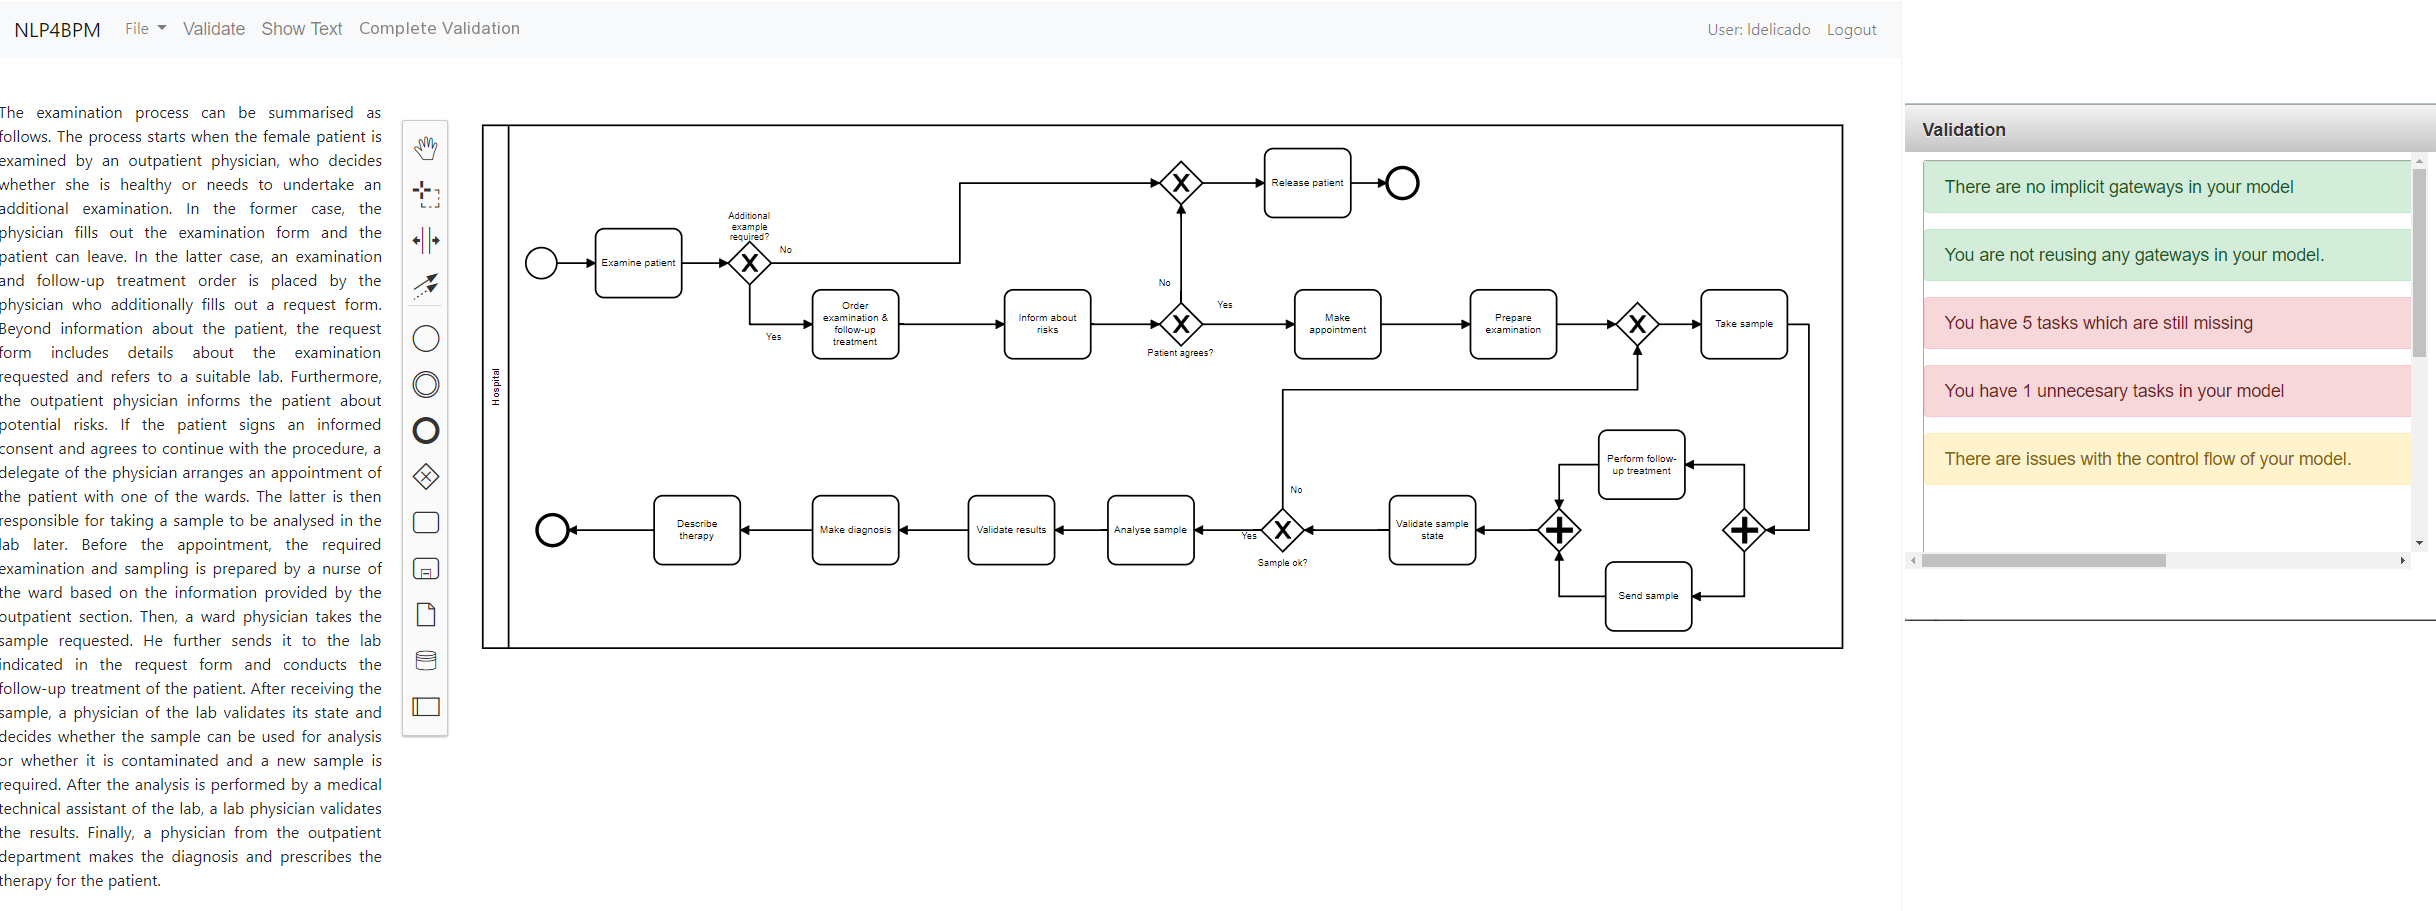
\includegraphics[width=\textwidth]{figures/validation}
  \caption{Model Judge modeling view}
  \label{fig:modeljudge_validation}
\end{figure}





\section{Approach}
\label{sec:modeljudge_approach}

At the Model Judge's core, there is the algorithm that produces a list of
diagnostics for their current business process model. The design and
implementation of this algorithm was implemented as a part of this Master Thesis.

In Figure~\ref{fig:modeljudge_overview}, we can see a BPMN diagram of the
diagnostic generation process. The inputs to the system are the \emph{Textual
  Description}, which corresponds to the exercise statement, and the
\emph{Process Model} created by the student. First, the textual description is
analyzed by the Text Annotation module (See \texttt{text2atd},
Section~\ref{sec:architecture}) to automatically produce an Annotated
Textual Description, which is then completed with human intervention to include
the domain expertise not available to the NLP algorithms. This step is only
performed once and can be used to evaluate any number of students in that
exercise. Once a particular student wants to validate a partial model, the
process model is sent to Model Judge. First, the process model is
analyzed: A \emph{behavioral profile} is computed, and \emph{semantic roles} are
extracted from the text labels in the model using a specialised chart parser.
After the model is analyzed, the \textit{alignment} between the process model
elements, such as activities or gateways and the annotations in the ATD is
established. Finally, using all the previous information, the process model is
checked against a textual description by the \emph{diagnostics} module.

\begin{figure}[htb]
  \centering
  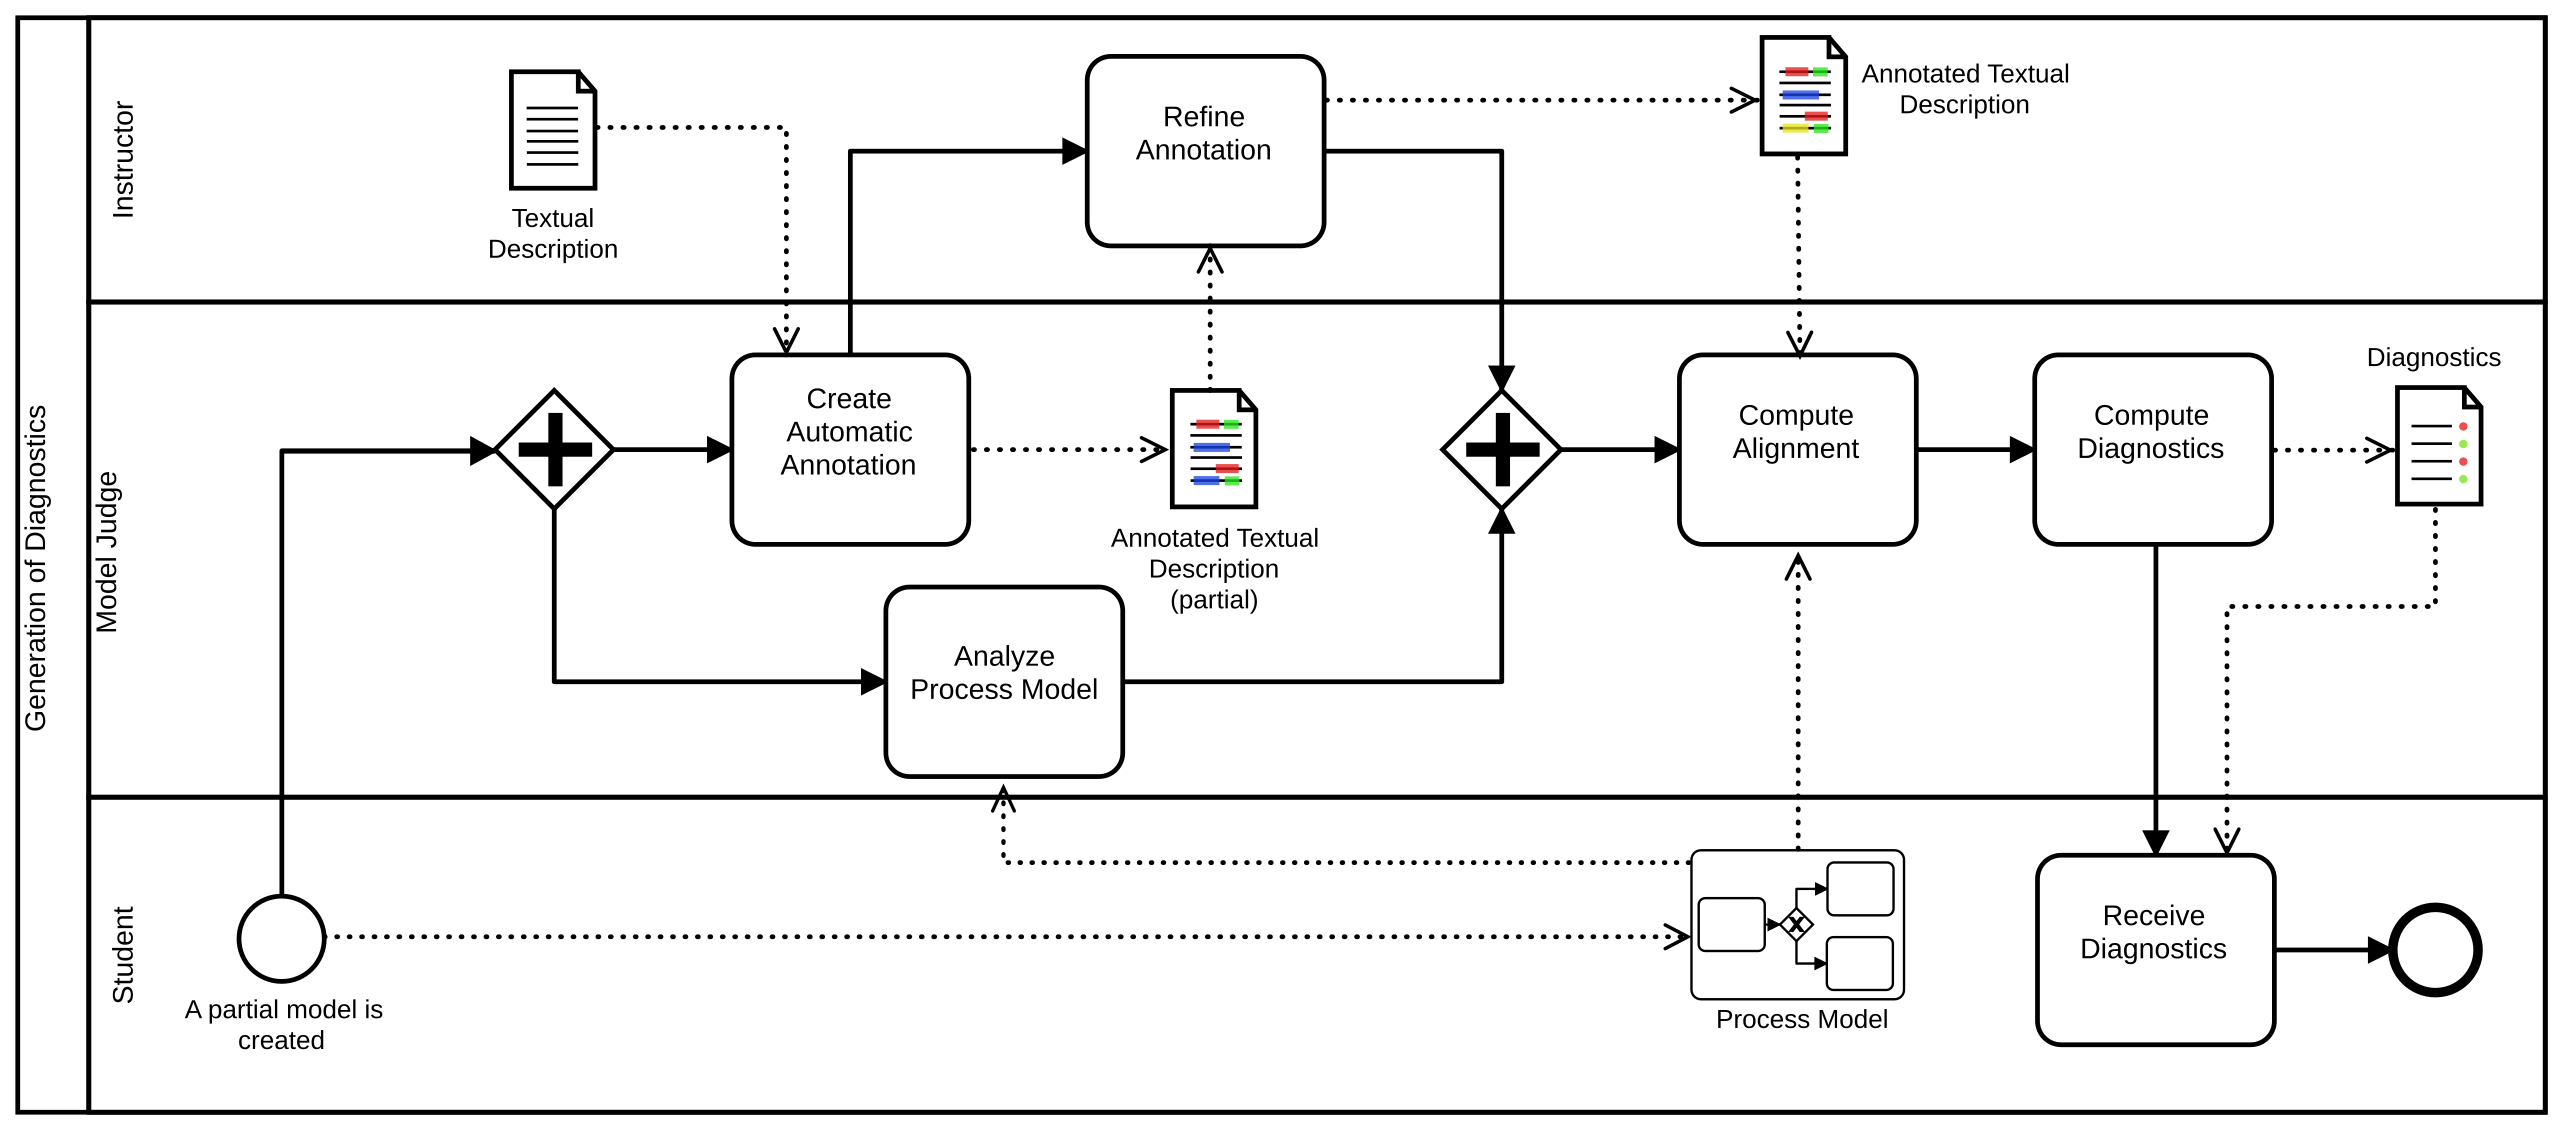
\includegraphics[width=\textwidth]{figures/overview_bpmn}
  \caption{\emph{Model Judge} process overview}
  \label{fig:modeljudge_overview}
\end{figure}

The next sections describe the multiple steps in Model Judge's algorithm
in more detail. Section~\ref{sec:process_model_analysis} covers the analysis of
the process model. In Section~\ref{sec:diagnostics_generation}, the necessary
steps for obtaining the diagnostics are computed. Finally, the details behind
the alignment of ATD and process models are discussed in
Section~\ref{sec:aligning_atd_bpmn}.
\todo{I don't like having alignment in its own section. However, the section is
  too long to be put in a subsection instead.}

\subsection{Process Model Analysis}
\label{sec:process_model_analysis}

Model Judge performs two separate analysis of a Process Model sent by a
student. First, a \emph{behavioral profile} of the process is computed, in order
to compare it to the one from the ATD during the alignment computation (See
Section~\ref{sec:alignment_creation}). The computation of a \emph{behavioral
  profile} has well known algorithms and can be performed as long as the
process' Petri net is \emph{bounded}\cite[Section IV.B]{murata1989petri}.
Analyzing a process model, thus, consists of three steps:
\begin{enumerate}
  \item Convert the BPMN process into a Petri Net, this somtimes results in
    unbounded Petri nets.
  \item Check the boundedness of the resulting Petri net, only if the
    property is fulfilled, the next step is executed.
  \item Compute the behavioral profile of the Petri net.  
\end{enumerate}

The necessary operations to compute the behavioral profile are implemented in
JBPT\cite{polyvyanyy2013towards}, a Java library consisting of several utilities
to manage business process models.

The second step in Model Judge's analysis of process models is extracting
semantic roles from its text labels from activities, gateways, events, swimlanes
and pools. Using FreeLing's generic parser and SRL module for this analysis,
however, has some drawbacks: NLP parsers are generally trained on large corpora
of written text, such as books or newspaper articles. However, this training
data doesn't represent well the kind of sentences found in a process model,
which are typically incomplete and use excessive
capitalization\footnote{Excessive capitalization happens when all the words in a
sentence are capitalized in order to highlight its importance. This is
considered good writing style in section headers or process model labels, but
most NLP parsers are not trained to recognise the phenomena and confuse some
words for proper nouns when it is used.}. A very common confusion of NLP tools 
when parsing text labels in models written in the english language occurs in the
case of noun-verb \emph{homographs}\footnote{Two words are \emph{homographs}
  when they share the same spelling}. Consider, for example, the phrase ``mail
confirmation''. A typical NLP parser would identify this as a noun phrase, the
\emph{confirmation of the mail}; this is because the \emph{prior} probability of
the ``mail'' word occurring as a noun is far higher in the typical training data
used. However, in business process models, labels usually start with a verb.
When consider this information, we see that the real meaning of the label is
that \emph{someone mails a confirmation}.

To deal with this, we built a custom SRL module which encodes the most common
label styles classified in \cite{leopold2013detection} in order to
build a chart parser specific to process model labels. Due to the simplicity of
most label structures, the parse tree can be directly used to extract the
semantic roles using a custom set of rules. In our current implementation, we
consider the most common types of labels:

\begin{description}
  \item[Verb-Object]{This label style consists of a verb in imperative form (the
      main \emph{action}), followed by a noun, representing the \emph{business
        object} and additional complements. For example, ``Examine patient'' is
      a label in Verb-Object style.}
  \item[Action-Noun]{In this label style, the main action is represented as a
      noun, and is usually preceeded by the business object. An example of this
      label style would be ``Patient examination''.}
  \item[Double-Action]{This is a compound structure, where two or more actions
    are described in a signle label, using Verb-Object style. ``Examine Patient
    and Request Sample'' could be an example label using that style.}
\end{description}

The grammar for the custom chart parser tries to ifentify any of the above
structures, and is written un such a way that that the root node of the parse
tree will be labeled with the identified writing style, if found. For example, a
label written in the \emph{noun-action} style will have this information
reflected at the root node of the tree. Using this grammar, the parsing is then
done as follows:

\begin{enumerate}
  \item {The $n$ most likely PoS-tag sequences of the label are computed.}
  \item {For each of the PoS taggings, the label is parsed using a chart
        parser with the aforementioned context-free grammar.}
  \item {If some parse tree's root is tagged with one of the aforementioned
      writing styles, the grammar the \emph{action} and \emph{patient} (i.e.
      business object) roles will be extracted by following the identified
      structure of the label. Note that due to BPMN's semantics, the
      \emph{agent} of the action is never described in the activity label, as
      that is the purpose of swimlanes.}
    
    
\end{enumerate}


\subsection{Diagnostics Generation}
\label{sec:diagnostics_generation}

The generation of the diagnostics is the final step in Model Judge's
algorithm. The goal is to generate human-friendly diagnostics by identifying the
differences between the ATD and the business process model. Most diagnostics can
be computed a two granularity levels. Either at a general level --e.g. The
process is missing \emph{some} activities--, or at a concrete level --e.g. The
process is missing a label about the ``Patient Examination''--. The computation
of the diagnostics uses the information in the ATD, the analysed process model
and the alignment between the two. In this section we detail which diagnostics
are currently generated by Model Judge and how they are computed.

\subsubsection*{Syntactic Diagnostics}
The computation of syntactic diagnostics only requires the
process model. Most checks implemented use well-known algorithms. Particularly,
checking the use of implicit gateways or gateway reuse consists of a very simple
structural check. On the other hand, the presence of non-natural loops can be
determined by checking for cycles in the process graph after removing all its
{\em back edges}, computed from the {\em dominator tree}~\cite{LengauerT79}.

\subsubsection*{Pragmatic Diagnostics}
The approach we use for checking adherence to a writing style is based on
using the custom  parser for labels described in
Section~\ref{sec:process_model_analysis}. Particularly, we use the
identification of the label writing style in the root of the label's parse tree
in order to restrict the labels to a certain set of accepted styles, which can
be configured.

In the current implementation, the writing style check focuses on looking
for double actions, that is, activity labels that consist of two actions, such
as \textit{``Close Ticket and Inform the Manager''}, for which the students are
encouraged to write two separate activities. However, this technique can be
adapted so any organization can enforce a label writing style in a flexible way.
This adaptation would consist of expanding the grammar to handle the newly
accepted new label styles, if necessary, and adding those styles to a list in
Model Judge's configuration files.

\subsubsection*{Semantic Diagnostics}
Semantic checks are concerned with the underlying process
semantics. Computing these diagnostics requires all the information from the
annotated textual description, the process model and the alignment.

To detect that an \emph{activity is missing} from the process model, the alignment
information is used. Particularly, if there is an action in the ATD with no
correspondences from the process model, the activity is missing from the process
model. The system can then inform the modeler by generating a detailed error
message using the annotated data from the textual description.

Detecting \emph{unnecessary activities} also relies on the alignment. In this case,
there will be a process model activity $p$ aligned to some ATD action $a$. If the
similarity between $p$ and $a$ is low enough, according to the result of
computing the predictor (as described in Section~\ref{sec:predictors}), the
activity is considered unnecessary, as there is no good match for the activity
in the text.

The \emph{coverage of roles} is computed similarly to activities. In this case, the
similarity function is used to assess the similarity between \emph{role}
annotations and the process model's swimlanes. An unrestricted alignment is
performed and the matches are used to detect missing and unnecessary roles as
previously described with activities.

Finally, in order to detect \emph{control flow consistency}, we focus on the
differences between the constrained and unconstrained alignment. Particularly,
if the objective function (that is, the sum of correspondence similarities)
between the two alignments differs greatly, a warning is displayed to the user
informing that the control flow in their process may be wrong. This careful
phrasing is intended, since our testing has shown this method to not be
completely reliable to detect subtle control flow errors, both in terms of
false positives and false negatives.



\section{Aligning ATD and BPMN Process Models}
\label{sec:aligning_atd_bpmn}

Establishing the correspondence between the annotations in the textual
description and the elements in the business process model is necessary in order
to compute some diagnostics, such as the semantic-related ones. The goal of this
computation is to be able to assess which parts of the process model have been
correctly modeled by the student, according to the textual description.

In order to achieve this goal, the technique presented in
\cite{10.1007/978-3-319-59536-8_26} is used, which computes an alignment from
process model activities to a textual description's sentences. The most
important adaptation is the alignment input, which now considers the ATD's
\emph{annotations}s instead of the plain sentences. In order to achieve this
goal, the \texttt{atd2fl} and \texttt{atd2bp} modules from \emph{ATDlib} are
used, in order to accurately transform the input text to a \emph{FreeLing}'s
semantic graph and \emph{behavioral profile}, which is the original expected
input of the alignment algorithm.

Figure~\ref{fig:alignment_overview} shows an overview of the alignment approach
presented in \cite{10.1007/978-3-319-59536-8_26}. Next, we cover each of the
steps in the algorithm, and the necessary addaptations that were performed to
use the algorithm as part of Model Judge:

\begin{figure}[htb]
  \centering
  \includegraphics[width=\textwidth]{figures/alignmentoverview}
  \caption{Overview of the alignment technique presented in \cite{10.1007/978-3-319-59536-8_26}}
  \label{fig:alignment_overview}
\end{figure}
\subsection{Feature Extraction}

%WIL: OVERVIEW FIGURE

In order to establish a distance metric for two essentially different sources, such as
an ATD and a BPMN Process Model, the elements in the two representations are
converted into a canonical representation, the \emph{Feature Vector}. Feature
vectors are extracted for each $Action$ or $Condition$ in the ATD, and each
\emph{process element} (i.e. \emph{activity}, \emph{gateway} or \emph{event}) in
the business process model

A feature vector $v \in \mathbb{R}^\infty$ is a sparse real vector computed in
an infinite dimensional space. Each of the dimensions of the space correspond to
a linguistic feature of the element. For instance, the first non-zero dimension
of some vector $v_e$ may represent that the agent of the element $e$ is
associated with a certain word. The strength of this association --i.e. the
\emph{weight} of the feature-- is indicated by the magnitude of the vector in
that dimension.

We will refer to each individual dimension as a \emph{feature instance}.
Additionally, we group conceptually similar feature instances in \emph{feature
  families}. Each feature family corresponds to all the parametrizations of a
certain linguistic feature:

\begin{description}
	    \item[$contains\_action(a)$]{This feature family denotes the actions
          contained in a step $p$ or sentence $s$. For instance, when comparing
          a process step ``\textit{Examine Patient}'' to the annotated sentence
          ``\textit{The process starts when the female patient is examined by an
            outpatient physician}'', we extract the action ``\textit{examine}''.
          This implies the extracted feature vectors from the ATD and process
          model would share a non-zero value for the \emph{feature instance}
          $contains\_action(examine)$}

        \item[$contains\_role\_word(w) ~\&~ role\_main\_word(w)$]{This feature
            family denotes the roles that execute steps in a process. The
            former feature, $contains\_role\_word$, is extracted for each word
            $w$ that is part of a role. For instance, the ``\textit{outpatient
            physician}'' actor comprises the two words ``\textit{outpatient}'' and
            ``\textit{physician}''. By contrast, we use the $role\_main\_word$
            feature to denote the main word of the role, typically represented
            as the main noun, e.g., to explicitly capture the word
            ``\textit{physician}''. This separation allows us to give a different
            \emph{weight} to the main word with respect to the others.}

       \item[$contains\_object\_word(w) ~\&~ object\_main\_word(w)$]{These
           features encode the same information for \textit{business objects} as
           the previously described features do for \textit{roles}.}

       \item[$contains\_lemma(l, pos)$]{This feature is extracted from the
           target text if it contains a word\footnote{Note that in all feature
             types stopwords are not considered.} with the lemma $l$ and
           part-of-speech $pos$. In case of ATD, this would correspond to all
           the words contained whithin the \emph{Action} and its related
           \emph{Agent} and \emph{Patient} \emph{Entity} annotations, if any.
           This feature has a lower abstraction level than
           the previous ones and is included as a fall-back solution
           whenever the actor, role or action cannot be determined due to
           natural language ambiguity in the process model. In those cases the
           algorithm works at the word level. For example, for the annotated
           sentence ``A ward physician takes the sample requested``, the
           features \textit{contains\_lemma(physician, noun)},
           \textit{contains\_lemma(take, verb)} \textit{contains\_lemma(sample,
             noun)} and \textit{contains\_lemma(requested, adjective)} will be
           extracted.}
         
       \item[$contains\_synset(s)$]{This feature is extracted whenever the
           WordNet synset $s$ appears in the text sentence. It captures the
           semantics of words to help identify similarity when synonyms are
           used. For example, the WordNet synset \textit{10020890-n} recognizes
           that ``\textit{physician}'' is a synonym of ``\textit{doctor}'',
           such as used in the running example.}

       \item[$contains\_hypernym(s)$]{This feature is extracted from a target
           text containing a word for which $s$ is an hypernym\footnote{A word
             $w_1$ is a \textit{hypernym} of $w_2$ iff $w_1$ describes a
             superclass of $w_2$ (e.g. \textit{mammal} is a hypernym of
             \textit{cat}, and \textit{document} is a hypernym of
             \textit{letter}). Hypernymy is obtained from WordNet.} at distance
           \emph{HL} or less. \emph{HL} is a parameter of the algorithm. In the
           running example, a hypernym of ``\textit{physician}'' is
           ``\textit{medical practitioner}'' (\textit{10305802-n})}
\end{description}

By using ATD, which are accurately annotated, this feature extraction phase is
improved. Particularly, the high level features from the text can be reliably
extracted for all \emph{Action}s, since they are available through the
\emph{Agent} and \emph{Patient} relations. This means the algorithm doesn't need
to rely as much on the word-based features.

\subsection{Similarity Computation}

Once the heterogeneous sources are converted into a canonical representation, a
standard similarity metric can be used to compare them. As shown in
\cite{10.1007/978-3-319-59536-8_26}, the metric that gives best results for our
problem domain is the \emph{Weighted Overlapping Index}, computed as:

\begin{equation}
  WeightedOverlapping(a, b) = \frac{a \cdot b}{min\{\Vert a \Vert^1, \Vert b \Vert^1\}}
\end{equation}

Where $\Vert v \Vert^1$ represents the L1 norm of the vectors.

\subsection{Alignment Creation}
\label{sec:alignment_creation}

The next step is the computation of the alignment between process model elements
and the annotations of an \emph{ATD}. The alignment contains the
corresponding ATD action for each activity, gateway and event of the process model.

\newcommand{\corresp}[2]{#1 \sim #2}
\newcommand{\ncorresp}[2]{#1 \nsim #2}

Formally, we define an alignment $\sigma$ to be a set of correspondences of the
form $\corresp{n_k}{a_i} ~ \text{ for some } n_k \in N, ~ a_k \in A$, where $N$
denotes the set of elements of a process model and  $A$ is the set of actions
of the ATD. 

In order to establish an alignment between process model elements and sentences,
we impose two types of constraints on the alignment:  \textit{cardinality}
constraints and \textit{ordering} constraints.

\begin{description}
\item[Process step-to-sentence cardinality.]{
    For process model activities and events, we enforce that each of them is
    aligned to exactly one ATD action, whereas we allow multiple steps to be aligned
    to the ATD action. This, accounts for an activity being described once in
    the text, but being duplicated in the model, due to some requirement in the
    control flow.}
\item[Process step ordering.]{Assuming there are no contradictions between the
    control flow of the ATD and the process model, we can restrict the set of
    possible alignments for those that would violate the natural order of the
    process. This is one of the points where Model Judge's approach
    differs from the technique described in \cite[Section
    5.6]{10.1007/978-3-319-59536-8_26}, where the temporal relations in the text
    could not be computed. By using accurately annotated ATD, we are able to
    extract a full \emph{behavioral profile} for the text. This allows us to set
    the restriction that, for each pair of correspondences, $a \sim s, a' \sim
    s'$, the temporal relation between $a$ and $a'$ is the same for sentences
    $s$ and $s'$. More formally expressed as: $\forall (a \sim s, a' \sim s')
    \in \sigma^2 : bp_{pm}(a, a') = bp_{atd}(s, s')$, where $bp_{pm}$ and
    $bp_{atd}$ are the behavioral profiles of the process model and annotated
    textual description respectively.
    
    However, this restriction can lower the quality of the alignment when there
    are consistency errors in the control flow of the process. That is why two
    alignments are computed in our approach. One with ordering restrictions and
    one where this set of restrictions is disabled.}
\end{description}

The optimal alignment is then found, which is the one that maximizes the sum of
the similarities of the alignments, while preserving the aforementioned
constraints. This problem can be solved in linear time where the \emph{ordering
  restrictions} are disabled, but becomes difficult when considering them. For
the latter case, we modelled the problem as an ILP optimization, which was found
to be fast enough for the use case of student evaluation\footnote{Using the
  Gurobi\cite{gurobi} ILP solver, an answer from the optimization can be found
  in less than a second, thus, the NLP analysis becomes the bottleneck of the
  process}.

\subsection{Predictor-based Refinement}
\label{sec:predictors}

This is one of the key steps in order to compute the \emph{unnecessary activity}
diagnostics in Model Judge. The optimal alignment described in the
previous section, is computed under the assumption that the process model and
the ATD describe the same set of process activities. However, this is not the
case when evaluating partial models performed by students. Particularly, the
following inconsistencies may result in an alignment that is incorrect:

\begin{enumerate}
  \item The student has modeled an activity which is not in the ATD, meaning it
    is not relevant to the process.
  \item The student has not modeled an activity which is in the ATD, meaning it
    is missing 
  \item The order in which the activities are described in the model 
\end{enumerate}

Model Judge works by considering the alignment in order to generate
its diagnostics corresponding to points \emph{1} and \emph{2}. This is explained
in further detail in Section~\ref{sec:diagnostics_generation}. However, the
alignment computed at this point is not sufficient to determine which
unnecessary activities the student introduced. The similarity scores of the
correspondences are higly valuable indicators in order to detect this
information. Because of that, we introduce a refinement step after the alignment
which consists in applying a threshold on the similarity function, to discard
the correspondences with very low similarity from the process.

In the refinement step, instead of applying the threshold directly to the
similarity function, we introduce the concept of \emph{predictors}. A predictor
is a function of the correspondences in the alignment which assigns a likelyhood
value of that correspondence being valid (i.e. not unnecessary). This value will
be always in the interval $[0,1]$, but does not represent a probability. In our
approach, we defined the following predictors:

\begin{itemize}
	\item \textit{p-sim}$(n \sim a)$: the likelihood that a correspondence $n \sim a$
    relates to an unnecessary activity, given as the similarity score between
    the step $n$ and the ATD action $a$~ i.e. $sim(n,a)$.
    
	\item \textit{p-rel-S}$(n \sim a)$: the value of the previous predictor,
    normalized by the maximum similarity between $a$ and any other process step,
    ~i.e. \\ $\frac{sim(n,a)}{max~\{sim(n', a)~|~n' \in N\}}$
    
  \item \textit{p-harm}$(n \sim a)$ The harmonic mean between \textit{p-sim}$(n,
    s)$ and \textit{p-rel-S}$(p,s)$
\end{itemize}


The choice of predictors is greatly influenced by the similarity function. In
our approach, the similarity function uses the \emph{Weighted Overlapping Index}
and thus is contained in $[0,1]$. However, in practice, we have observed that
depending on how different is the level of verbosity in the text and model, the
similarity functions will vary overall. This motivates the coice for a relative
predictor, which won't be affected by the differences of the discourse in the ATD and
process model. However, using a relative predictor alone like \textit{p-rel-S} would
fail in the event that all the activities introduced by the user are
unnecessary. In order to have a predictor that is robust to such scenarios, we
take the harmonic mean between \textit{p-rel-S} and \textit{p-sim}, using
\textit{p-harm} as the predictor for Model Judge


 



\section{Experiments}
\label{sec:modeljudge_results}

%\todo{Describe dataset in further detail}

Model Judge has been tested in two separate modeling courses. The first was performed on the Technical University of Denmark (DTU) during February 2018. as part of a graduate course on business process management. 
The second course was performed at the Catholic University of Santa Mar\'ia (UCSM) in Peru during March 2018 as part of a practical session in the Business Process Management course in the Computer Science degree.

In order to validate how the Model Judge helps novice modelers, we performed two evaluations.  The first one consisted in analyzing the recorded data from the modeling sessions (Section \ref{sec:data_analysis}). The second evaluation arises from a survey that was handed to the students at the end of the modeling course (Section \ref{sec:questionaires}). Below, we detail the results obtained in both evaluations.

\subsection{Analysis of the Modeling Session Data}
\label{sec:data_analysis}
There were substantial differences in the setting of the two courses. On the DTU course, students were allowed to complete the exercise at home without a time limit. On the other hand, the UCSM course consisted in two exercises that had to be completed in a two-hour session.
%Additionally, in first UCSM exercise, the students were discouraged to use the complete validation functionality until the end of the exercise.
Additionally, some technical issues affecting DTU students were corrected before the UCSM course. Despite the differences, we believe the information recorded is still relevant for the analysis we present in this session. 
%However, we believe a better controlled experiment would be necessary in order to draw more statistically robust conclusions.
%\todo{[JS: Please check the above paragraph.]}

% For the students that allowed the recording of their data for research purposes 
For every student, we stored periodically (every minute) information for the whole modeling session. Additionally, information was also saved each time the user performed a simple or complete validation. In particular, we recorded a total of 8410 intermediate models for 72 students. For the snapshots, we stored: \textit{(i)} A unique user identifier. \textit{(ii)} The process model in BPMN (XML) format. \textit{(iii)} The timestamp of the snapshot. \textit{(iv)} The type of information: automatic, validation or complete validation. \textit{(v)} The validation results of our tool for the particular process model. Note that the validation results were computed for all snapshots, despite the students only seeing the ones they explicitly requested. 
After the modeling course ends, we analyzed the snapshots with the aim of observing the evolution of the number of validation errors during the modeling sessions. The dataset used to perform this analysis can be found in the following address: \texttt{\url{http://www.cs.upc.edu/~pads-upc/ModelJudgeData.zip}}.

\subsubsection{Modeling Behaviours}

By manual inspection, we identified several modeling profiles when analyzing the sessions data.
Figure~\ref{fig:profiles} shows a representative for each of the identified profiles, when plotting number of validation errors vs.
time (in seconds)\footnote{There exists few outlier profiles that do not match any of the three representatives shown in Fig.~\ref{fig:profiles}.}.
An instructor can have a good summary of the student evolution by looking at these student's plots:
\emph{(i)} The first group is composed of students that frequently use the validation and complete validation functions, and ended up with almost no bad diagnostics. This group corresponds to $19.0\%$ of the students ($30.4\%$ in the DTU course and $12.5\%$ in the UCSM course).
\emph{(ii)} The students from the second group frequently use the simple validation, however, only check the complete validation at the end of the session. The final amount of bad diagnostics for this group is comparable to the previous one. This group corresponds to $60.3\%$ of the students ($56.5\%$ in the DTU course and $62.5\%$ in the UCSM course).
\emph{(iii)} The students from the third group started working on the exercise but finished before fixing the majority of bad diagnostics. We have observed that the students in this group performed substantially less validations. This group corresponds to $20.6\%$ of the students ($13.0\%$ in the DTU course and $15.8\%$ in the UCSM course).

\begin{figure}
  \centering
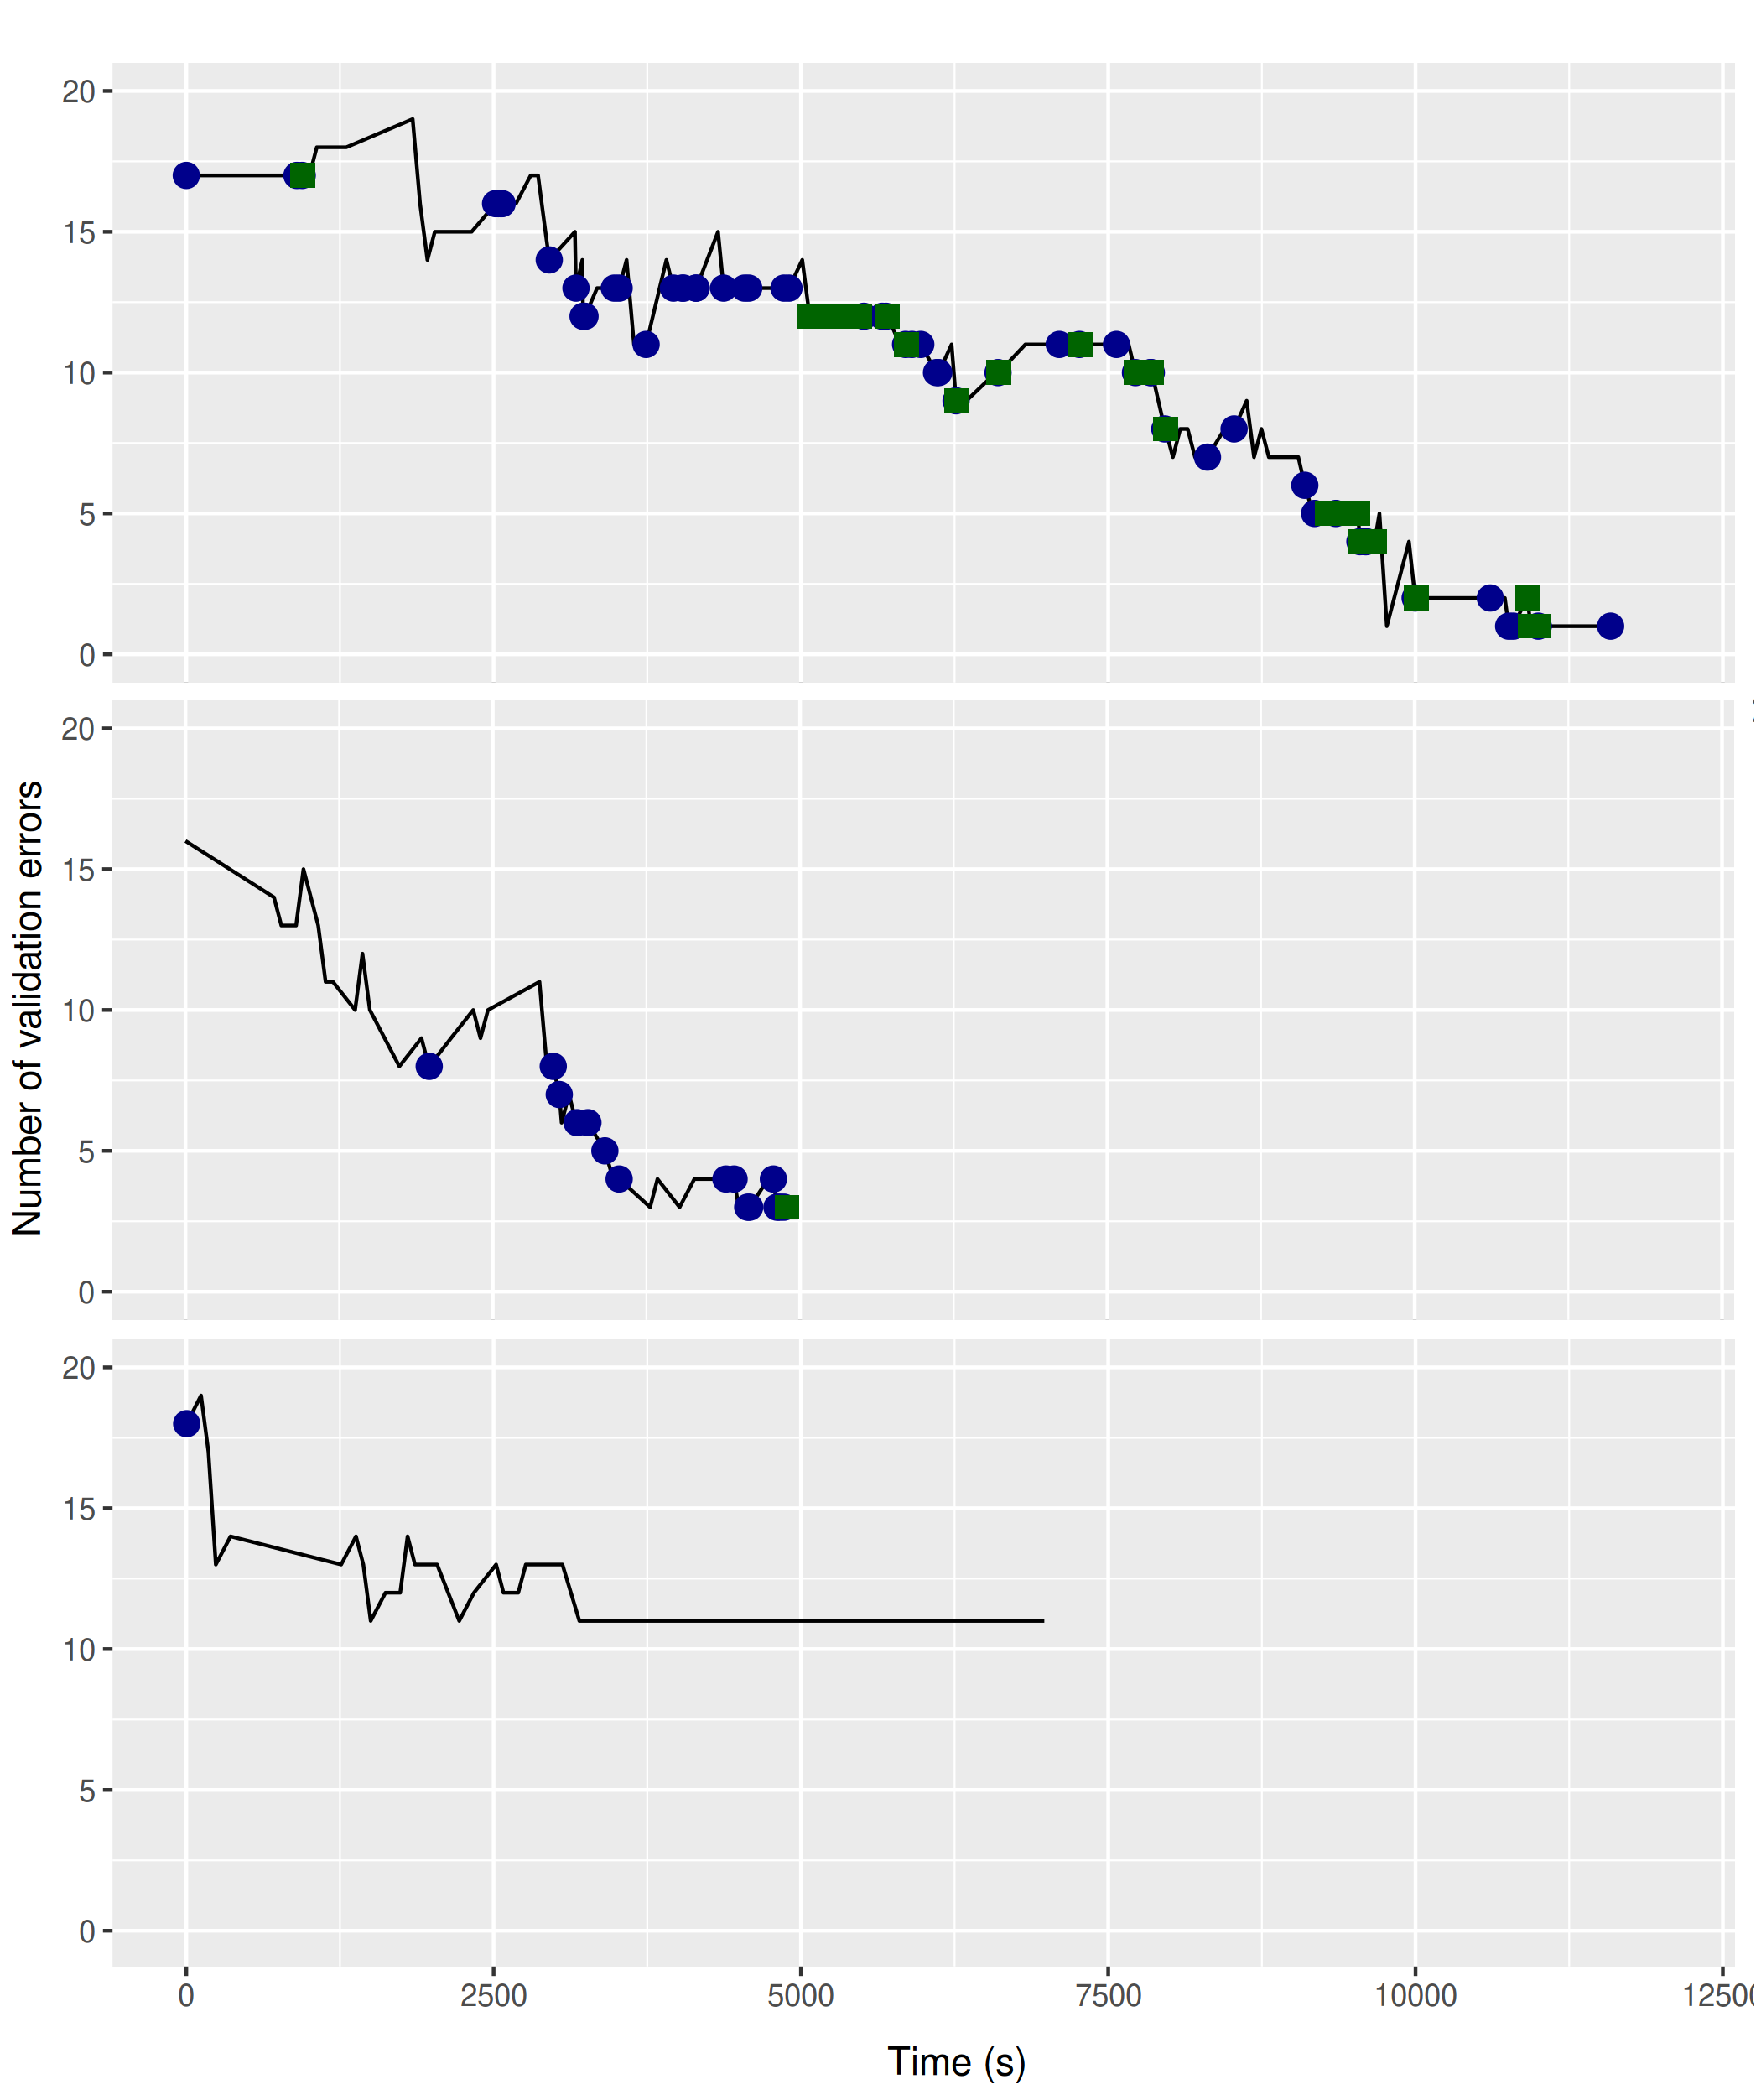
\includegraphics[width=0.85\textwidth]{figures/results/profiles.png}
\caption{Three characteristic behaviors observed in the modeling sessions. The blue circles represent simple validations, while green squares denote complete validations.}
\label{fig:profiles}
\end{figure}

\subsubsection{Evolution of Diagnostic Types}


\begin{figure}
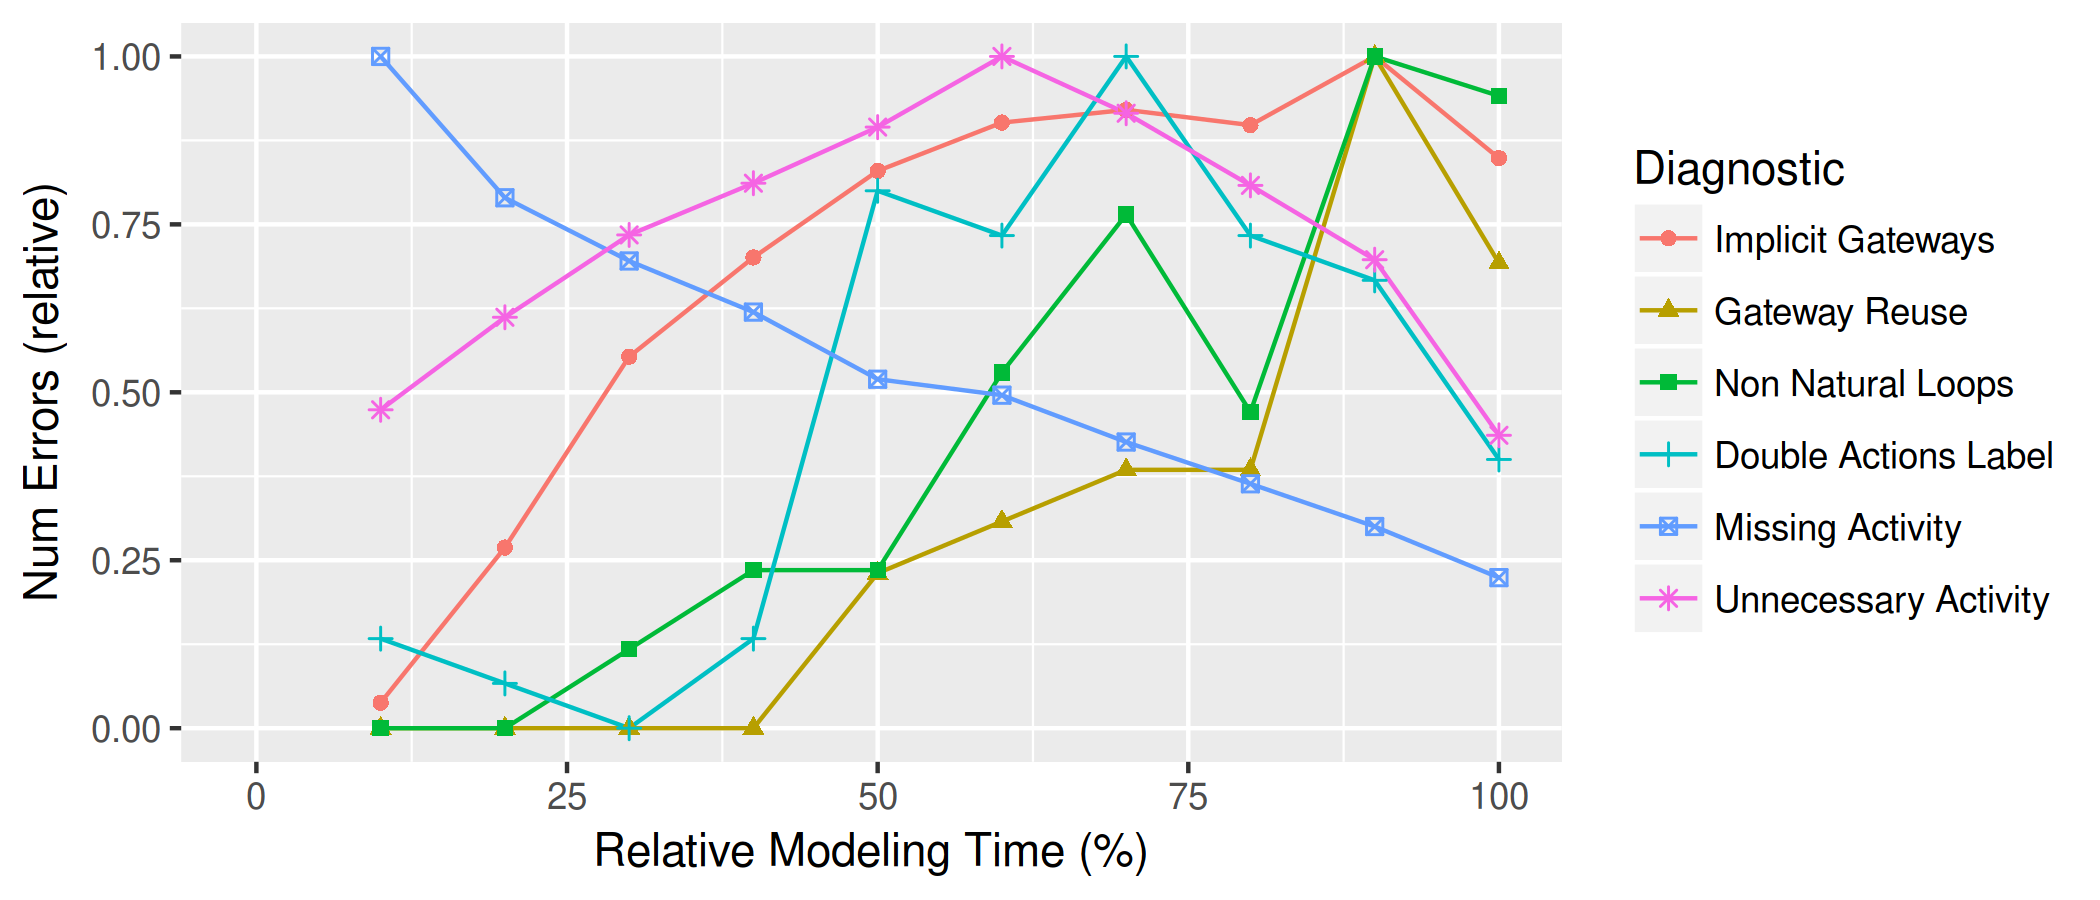
\includegraphics[width=\textwidth]{figures/results/evolution}
\caption{Evolution of the diagnostic types for the modeling session.}
\label{fig:error_evolution}
\end{figure}
\begin{figure}

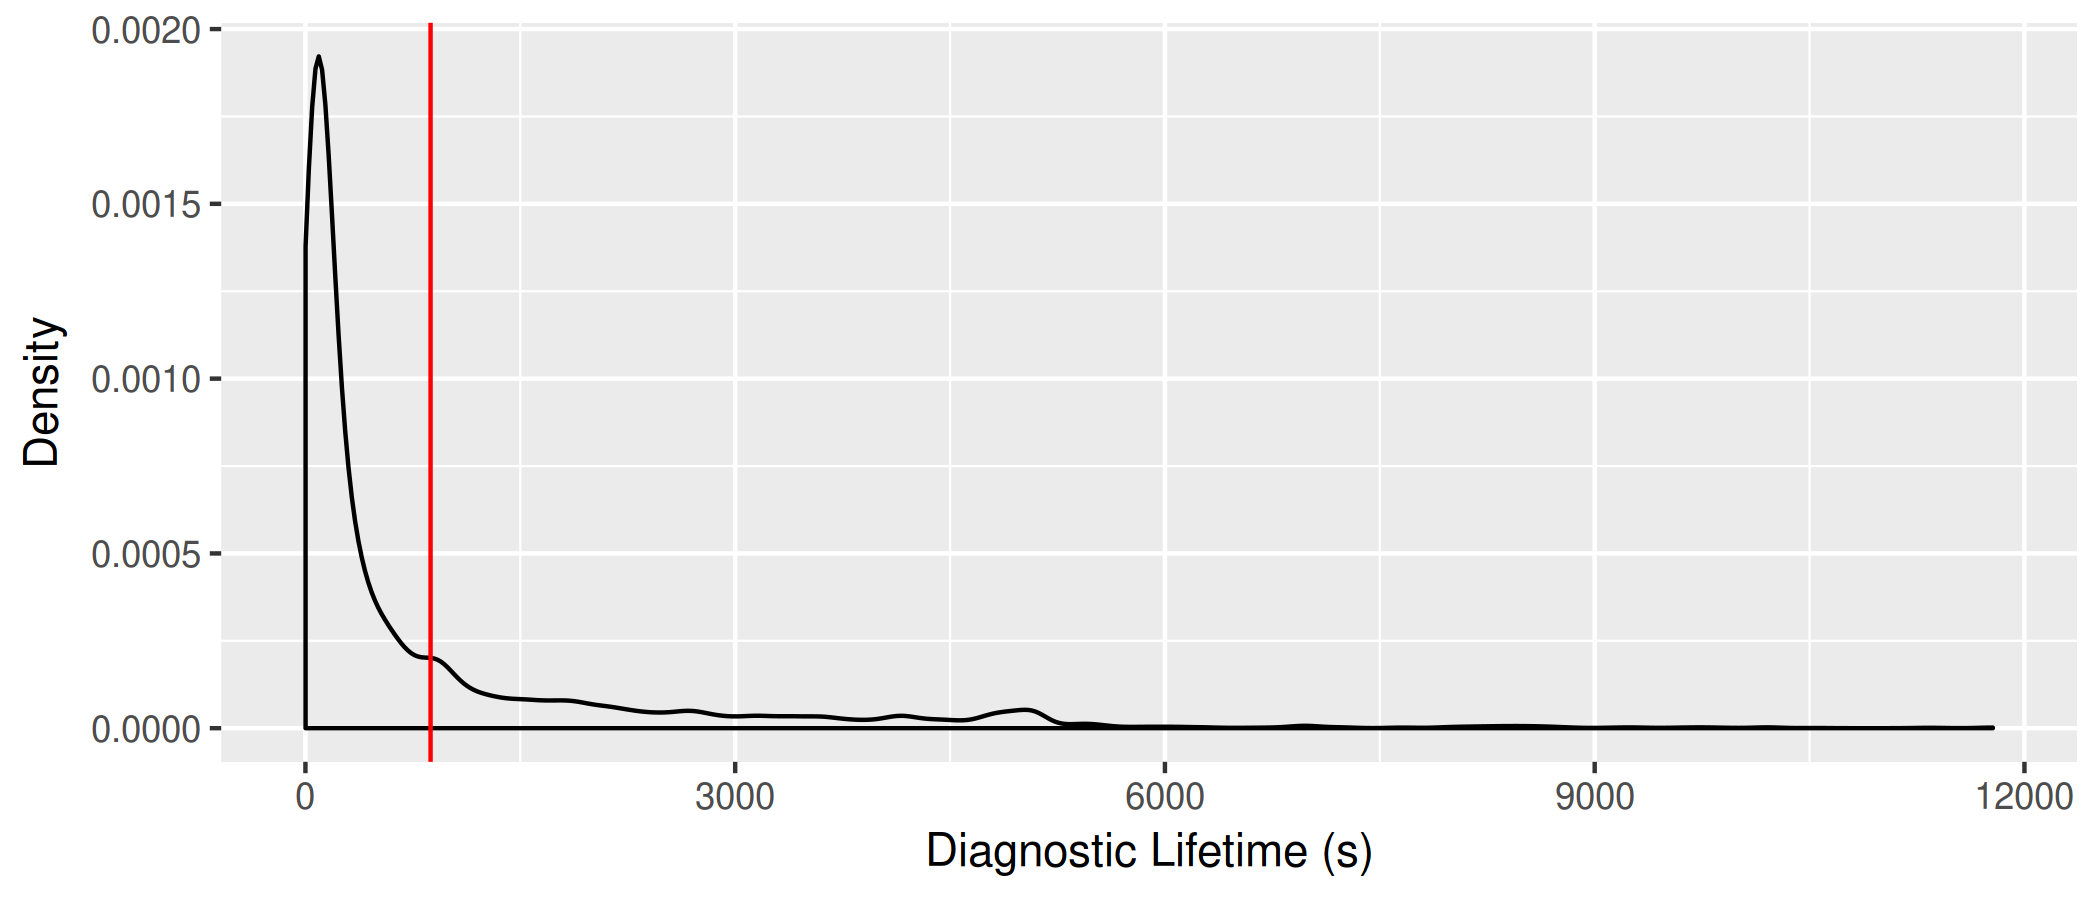
\includegraphics[width=\textwidth]{figures/results/lifetime_density.png}
\caption{Density plot of the diagnostic lifetimes variable.}
\label{fig:avg_lifetime_distribution}
\end{figure}

\begin{figure*}
  \centering
	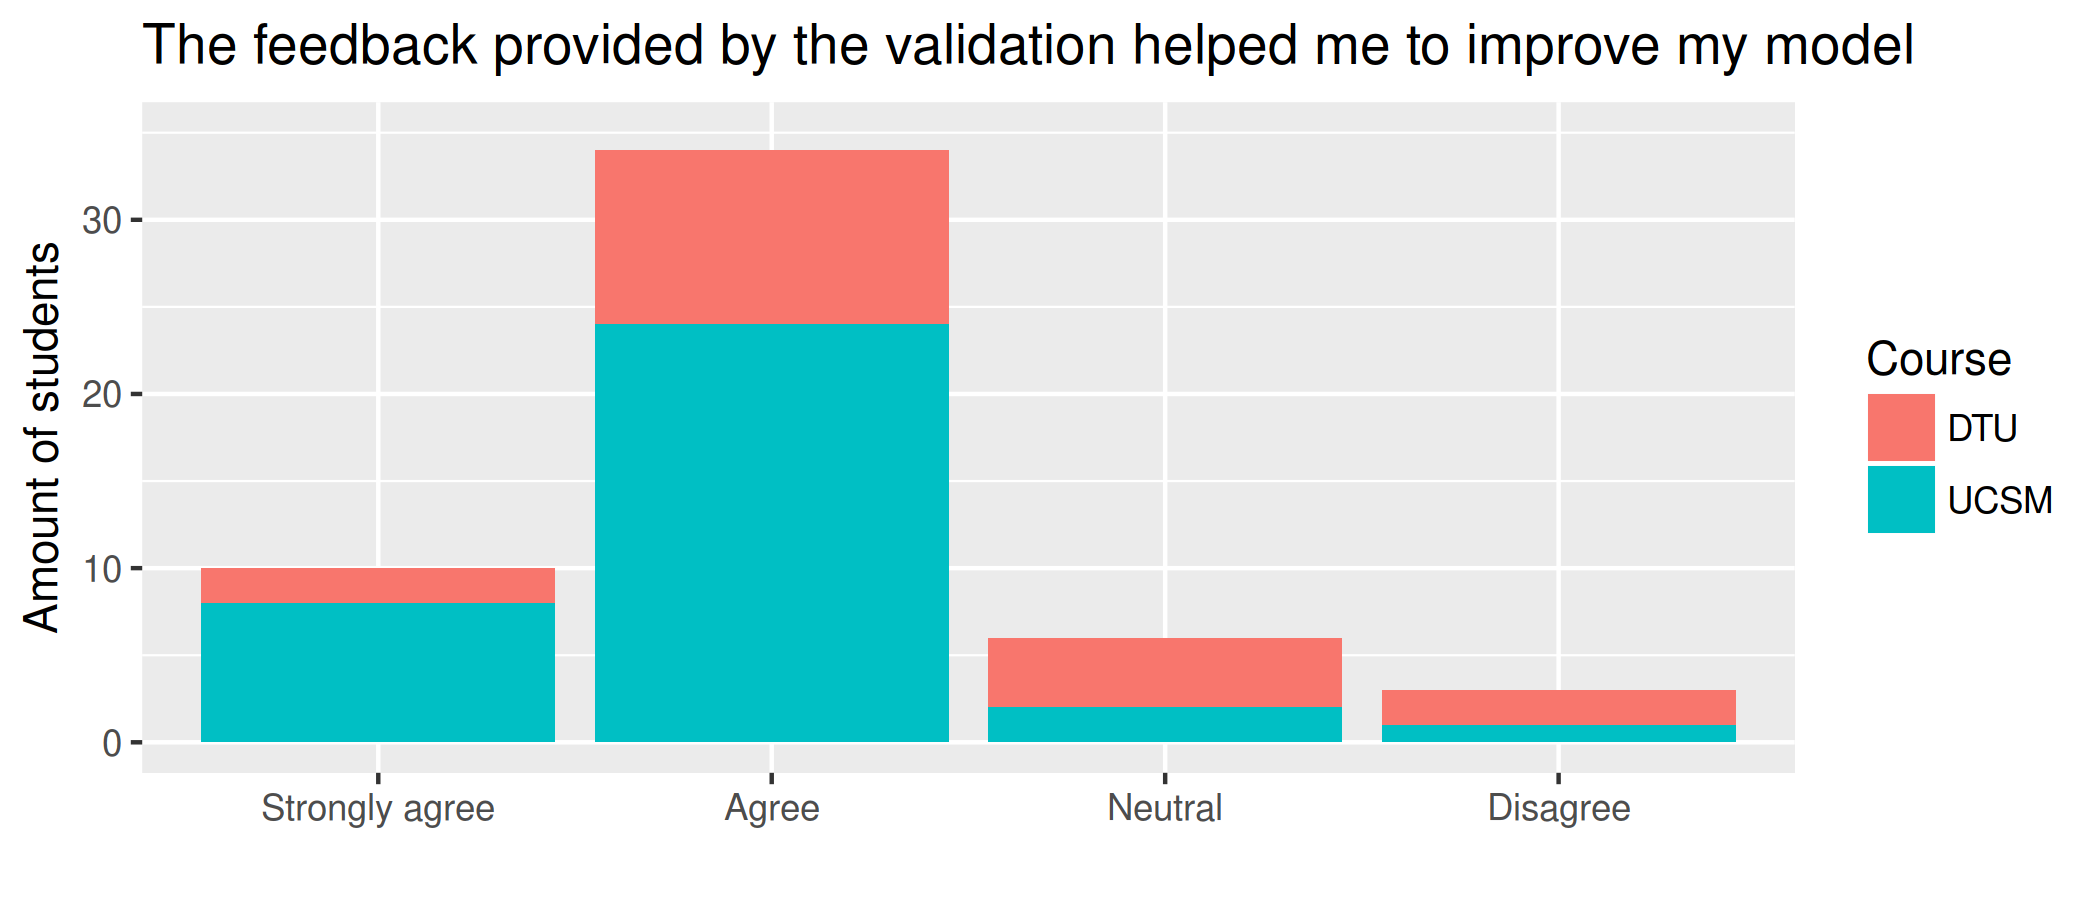
\includegraphics[width=0.9\textwidth]{figures/results/validation_helped_improve}
  \vspace{5pt}
  \newline
  \noindent
	\centering 
	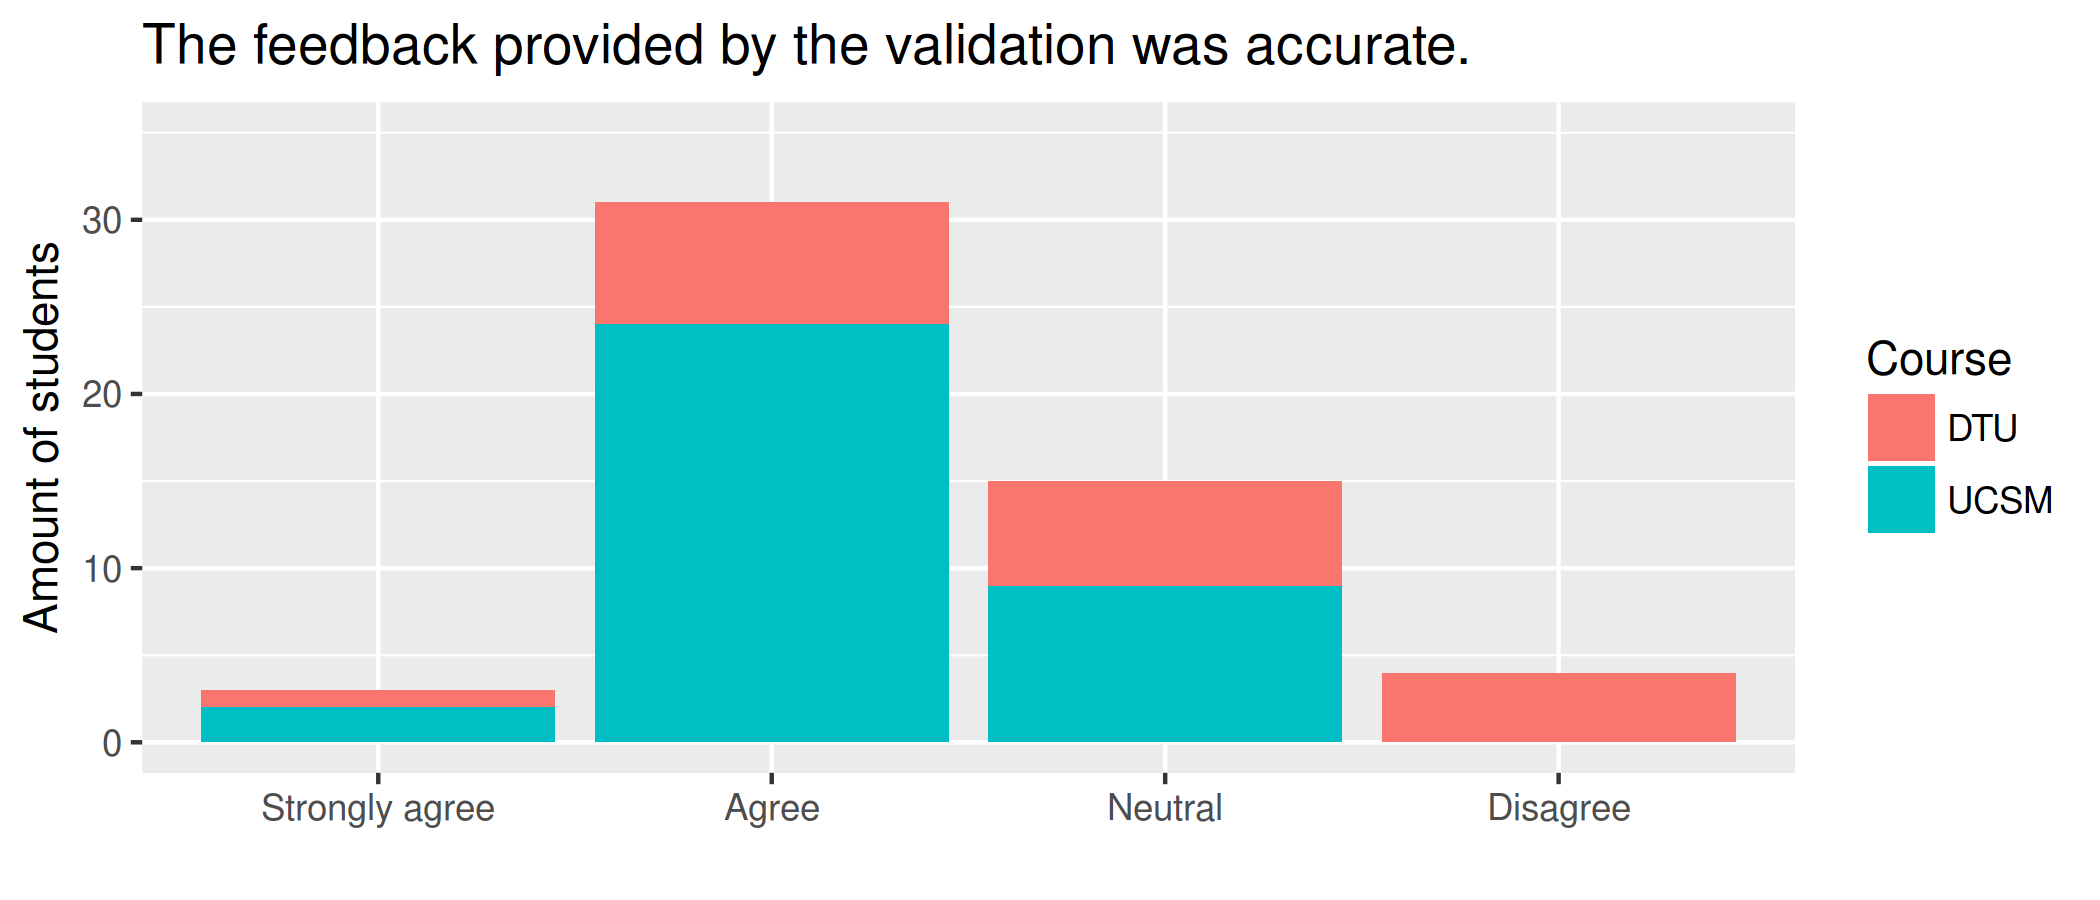
\includegraphics[width=0.9\textwidth]{figures/results/validation_was_accurate}
  \vspace{5pt}
  \newline
  \noindent
	\centering 
	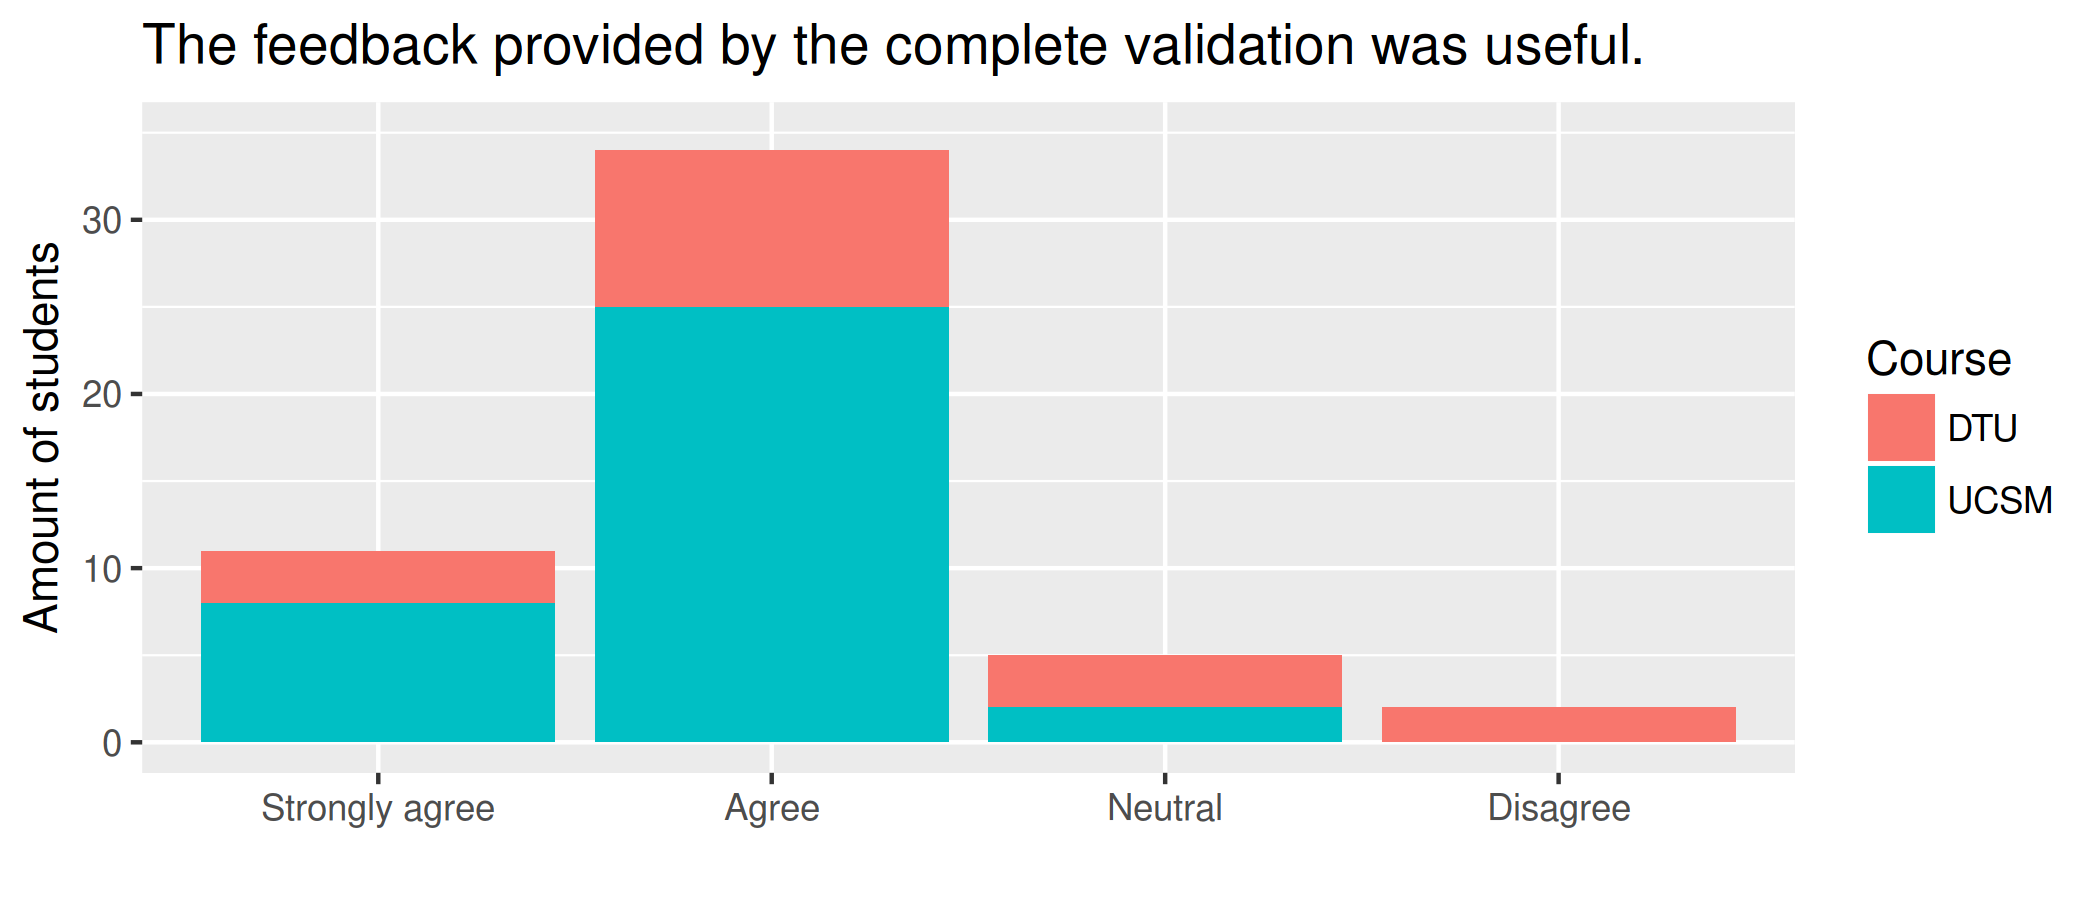
\includegraphics[width=0.9\textwidth]{figures/results/final_was_useful}
  \vspace{5pt}
  \newline
  \noindent
  \centering 
  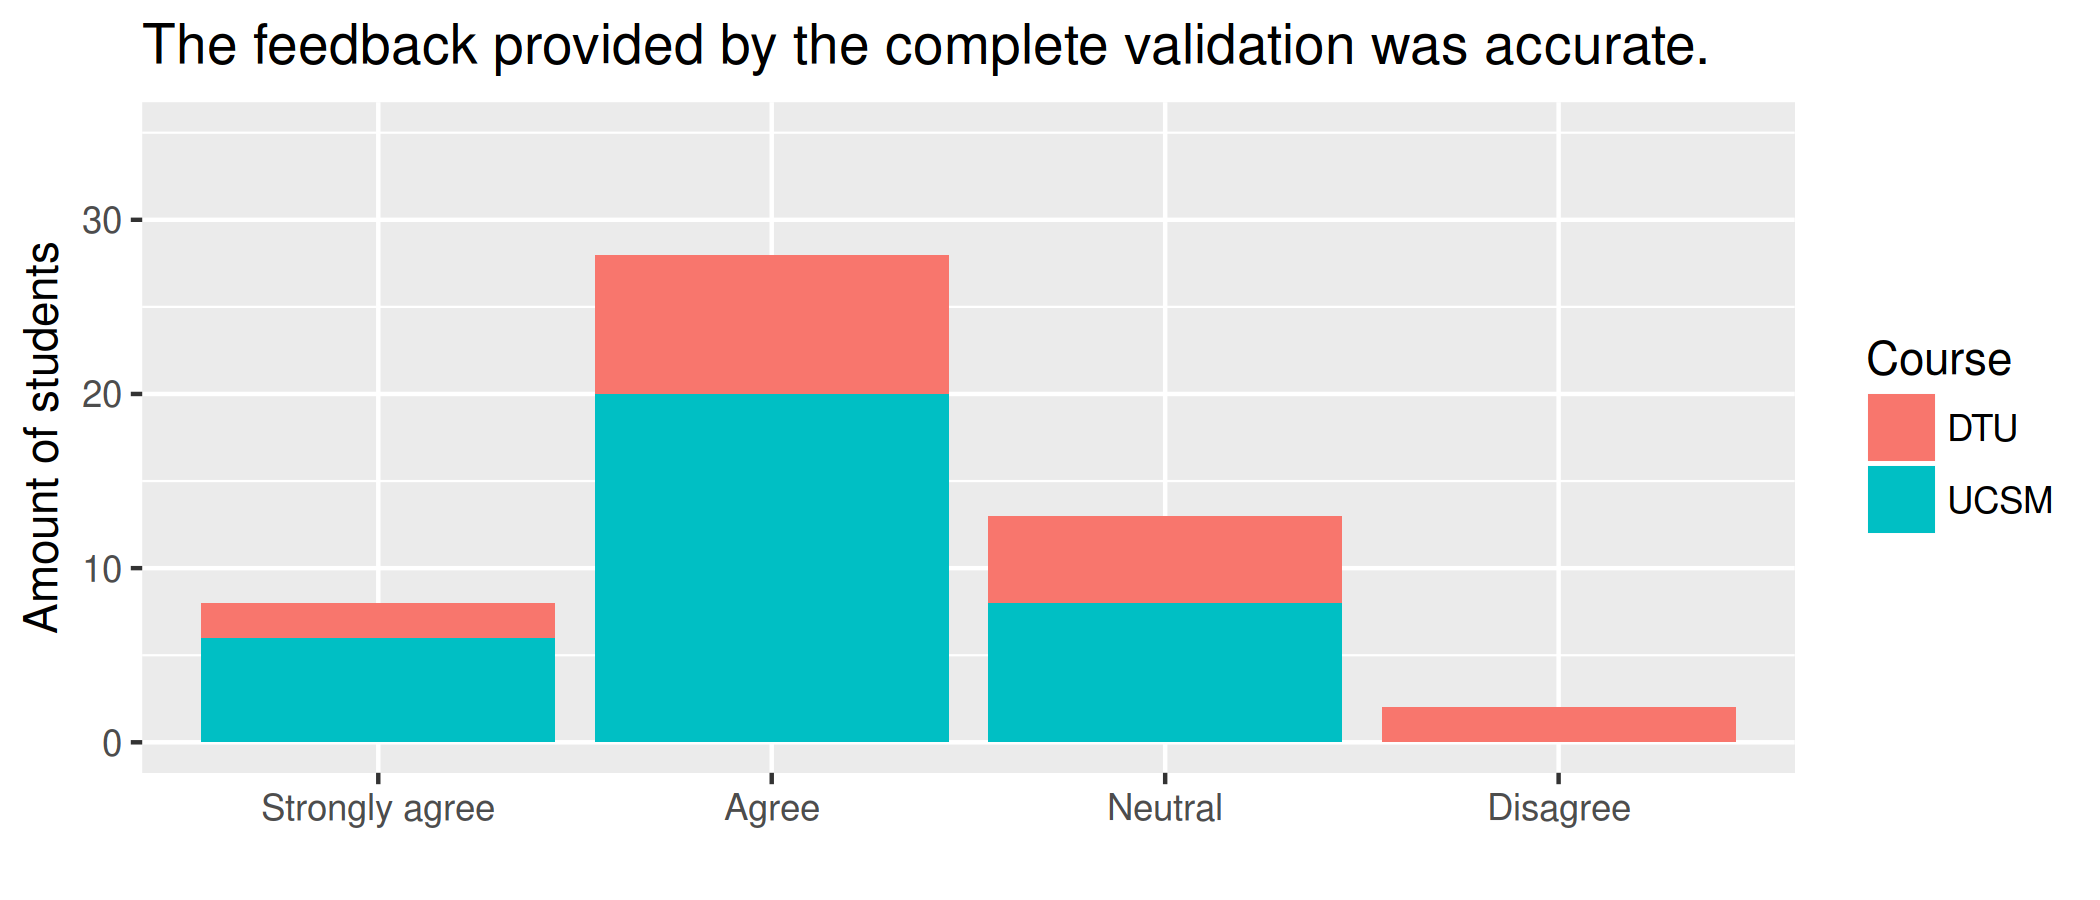
\includegraphics[width=0.9\textwidth]{figures/results/final_was_accurate}
\caption{Results of the student survey for the modeling courses.}
\label{fig:survey-results}
\end{figure*}

\newcommand{\expnumber}[2]{{#1}\mathrm{e}{#2}}

We analyzed how the frequency of different diagnostics varies during the session. Figure~\ref{fig:error_evolution} shows the evolution of the average amount of diagnostics for all students, per diagnostic type. To better observe the relative behaviour of each type regardless of the amount of diagnostics in the category, we plot the values relative to the maximum of each category. We have encountered substantial differences between diagnostic types. 
Missing Activity diagnostics decrease as the session advances, since less activities will be missing as the modeling session progresses.
Unnecessary Activity and Double Action Writing Style increase for the first half of the session, then decrease. This behavior is consistent with the fact that most students do not start using the complete validation feature until the second half of the session. The more detailed feedback of the complete validation then helps them finding the more subtle errors in their process model.


The remaining diagnostic types have an oscillatory behaviour, but still increase for the duration of the session. This can be explained by the fact that, as the model session progresses, there is a greater chance of a student introducing an error leading to one of these diagnostics. However, the drops after 75\% progress could indicate that some students delay the correction of this errors until the end of the modeling session.

%-------------------
\subsubsection{Lifetime of the Diagnostics}
To get a deeper insight into the modeling session data, we computed the lifetime of the diagnostics given to the students. We define the diagnostic lifetime as the elapsed time between the moment a student introduces a mistake in the model, and the moment that mistake is corrected. Note that this metric is independent of the validations made by the student, since diagnostics are computed for all snapshots regardless of the student used the validation function or not.
The average lifetimes follow a long-tailed distribution (Figure~\ref{fig:avg_lifetime_distribution}). That is, in the average case mistakes are quickly corrected by the students. However, for a few cases, it can take a very long time to solve those mistakes. 

%An instructor can use the  information provided in Table~\ref{tab:avg_lifetimes} with several purposes, e.g., to 
%try to improve students understanding of the long-lasting mistakes.

%\todo{[JS: What could we say about the error lifetimes?]}

%\begin{table}
%\begin{tabular}{l|c}
%\hline
%\textbf{Diagnostic} & \textbf{Average Lifetime (s)} \\
%\hline
%Implicit Gateways & 1393 \\
%Gateway Reuse & 418 \\
%Non-Natural Loops & 393 \\
%\hline
%Double Actions Label & 891 \\
%\hline 
%Missing Activity & 2116 \\
%Unnecessary Activity & 367 \\
%\hline
%\textbf{Total} & 873s \\
%\hline
%\end{tabular}
%\caption{Average lifetimes for different error types}
%\label{tab:avg_lifetimes}
%\end{table}







\subsubsection{Relation of Number of Validations and Errors}

Finally, we studied whether there was a correlation between the number of validations performed by the students, and the number of bad diagnostics obtained. To that end, we performed a Pearson's correlation test on the following variables, measured for each modeling session: $V_s =$ ``Number of validations'', $V_c =$ ``Number of \textbf{complete} validations'', $D_{avg} =$ ``Average number of bad diagnostics during the modeling session'', $D_{end} =$ ``Number of bad diagnostics at the end of the exercise''.
\begin{table}
{\scriptsize
\begin{tabular}{l|c c c| c c c }
& \multicolumn{3}{|c|}{\textbf{Correlation Coefficient}} & \multicolumn{3}{|c}{\textbf{Test p-value}} \\
& \textbf{DTU} & \textbf{UCSM} & \textbf{TOTAL} & \textbf{DTU} & \textbf{UCSM} & \textbf{TOTAL} \\
\hline
$V_s$ \textasciitilde $D_{avg}$ & -0.693 & -0.626 & -0.664 & $8.77\times10^{-5}$ & $9.04\times10^{-8}$ & $3.33\times10^{-12}$ \\
$V_s$ \textasciitilde $D_{end}$ & -0.636 & -0.498 & -0.558 & $4.74\times10^{-4}$ & $5.07\times10^{-5}$ & $2.34\times10^{-8}$ \\
$V_c$ \textasciitilde $D_{avg}$ & -0.540 & -0.305 & -0.443 & $4.42\times10^{-3}$ & $1.77\times10^{-2}$ & $ 1.91\times10^{-5}$ \\
$V_c$ \textasciitilde $D_{end}$ & -0.219 & -0.406 & -0.397 & $3.85\times10^{-2}$ & $1.27\times10^{-3}$ & $1.57\times10^-4$ \\
\hline
\end{tabular}}
\caption{Pearson's correlation test results for the relevant pairs of studied variables (shown per course and total).}
\label{tab:correlations}
\end{table}
Besides the obvious correlations $V_c$ \textasciitilde $V_s$ and $D_{avg}$ \textasciitilde $D_{end}$, we also found strong negative correlations between the two pairs of variables, as seen in Table~\ref{tab:correlations}. That is, when the number of validations grows, the number of errors decreases. While all the correlations were statistically significant, we can see how the ones concerning the number of complete validations are weaker than the other two. %This can be explained by the fact that a subgroup of students were told to perform exactly one complete validation. %in one of the exercises. 
This can be explained by the fact that a large group of students did not use the complete validation, or did so only at the end of the session without addressing the feedback, while almost all students used the simple validation.
Additionally, we observed that the correlations found for the individual courses are less strong than considering the 72 students as one group.  

% \todo{[JS: I don't think we should draw very strong conclusions here. The fact that there is a correlation between the number of errors and the number of validations only indicates that the tool \textbf{may} (correlation != causation) help students achieve less errors. However, the statement that our feedback helps the students make better models cannot be drawn from this. The reader has to believe our feedback is accurate and useful (which is, more or less, backed by the surveys) for this correlation to indicate something good. If our feedback were to be counter-productive to model quality, the same correlation would indicate that our tool helps students achieve worse models.]}



\subsection{Student Survey}
\label{sec:questionaires}

In the survey, the students were asked demographical information, native language and line of work, as well as their degree of agreement on some aspects of the application with four questions, aimed at independently evaluating the accuracy and usefulness of the validation and complete validation functionalities. Finally, the students also were asked to write down any complaints and/or improvement suggestions.
% \todo{[JS: I found no interesting correlations with the demographic information so I left it out. Should we include it anyway?]}
Figure~\ref{fig:survey-results} shows the results of the survey: 
%As we can see from the results, 
a majority ($75.4\%$ in average) of students either agreed or strongly agreed in all questions. So we can say that the general perception is that using our framework was beneficial to the students. 
%\todo{[JS: Should we add that the instructors have also found the models to be of better quality with respect to previous years?]}.

When looking separately at the questions regarding \emph{usefulness} versus the ones regarding \emph{accuracy}, we can see a difference, with the students having a stronger level of agreement with the usefulness ($84.0\%$ on average) than accuracy ($67.0\%$ on average). We can thus conclude the student's perception was that the tool was useful, but not as accurate. This can be validated from the student's written suggestions, where in some cases they complained about the tool not understanding their process model labels.

By comparing independently the results of the two modeling courses, we can see the students from DTU were more critical with the tool ($58.3\%$ on average either agreed or strongly agreed) than the ones from UCSM ($83.6\%$ on average). We believe this difference can be partly explained by the presence of some technical issues during the DTU modeling course that were fixed for the UCSM one.


